%% LaTeX-Beamer poster template for KIT design
%% by Erik Burger, Christian Hammer
%%
%% version 1.2
%%
%% mostly compatible to KIT corporate design v1.2
%% http://www.uni-karlsruhe.de/download/uka/Gestaltungsrichtlinien_komplett.pdf
%%
%% Problems, bugs and comments to
%% burger@kit.edu

\documentclass{beamer}

%% Fill in the page size here. If the proportions of the fonts
%% are not satisfactory, change the scale parameter
\usepackage[orientation=portrait,size=a0,scale=1.4]{beamerposter}
\usepackage{multicol}
\usepackage{makecell}
\usepackage{color, colortbl}
\usepackage{textcomp}
\usepackage{pgfplots}
\usepackage{pgfplotstable}
\usepackage{subfigure}
\usepackage{overpic}
%\usepackage[demo]{graphicx}
\usepackage{graphicx}
\usepackage{ragged2e}
\usepackage{booktabs}
\usepackage{multirow}
\usepackage{blindtext}
\usepackage{biblatex}
\addbibresource{Bibliography/bibliography.bib}

\renewcommand*{\bibfont}{\scriptsize}

% \usepackage{capt-of}
\setbeamertemplate{caption}[numbered]

%weiß ich nicht \usepackage{filecontents}
\usepackage{tikz} 

\mode<presentation>{\usetheme{kitposter}}

\title[Short title]{Miniature (Medical) Robotic Systems \\ \Large Seminar Robotics in Medicine / Proseminar Informatics in Medicine SS 20\\ [.4em] }
\author{Johannes Häring}

\institute{\textbf{Institute for Anthropomatics and Robotics - \\[.2em]
Health Robotics and Automation}\\[.4em]
Engler-Bunte-Ring 8\\[.2em]
76131 Karlsruhe\\[.4em]
\href{http://hera.iar.kit.edu}{http://www.hera.iar.kit.edu}}

\begin{document}
% change the following line to "ngerman" for German style date and logos
\selectlanguage{english}

\begin{frame}
\frametitle{Seminar}
\Large 

\begin{columns}[] % align columns
    \begin{column}{0.45\textwidth}
        \begin{block}{\LARGE Abstract}
            \justifying \normalsize 
            Manual micro surgeries depending highly on the accuracy of the surgeon. This issue can be solved with miniature robotic systems. Micro robots are used in the neurosurgery, ophthalmic and pregnancy help. For navigating in narrow spaces in the brain a semi-flexible tool shaft is used. The tool shaft consists of springs and disks made of shape memory. The flexibility of the springs can be controlled by heat. Possible tool tips for manipulating tissue are micro scissors and milli grippers. The scissor blades are made of thin titanium sheets connected with a spring. The milli gripper is made of shape memory alloy. Both of them are actuated with an external magnetic field. For retinal surgeries completely flexible tools are used due to less displacement of the fiber network. In the area of pregnancy help a micro robot is used for navigating and holding an embryo in a for implantation suitable area for increasing the pregnancy probability. The miniature robots are teleoperated. The surgeons movement is processed with a computer which then actuates the robot. This allows removing the tremble and increase the accuracy. An issue with teleoperated systems is the missing tactile feedback. First automation approaches are made with an automatic collision avoidance algorithm or the real time tool detection. Also first algorithms are developed for preplanning the surgery.
        \end{block}    
        
        \vspace*{20pt}
        
        \begin{figure}
            \centering
            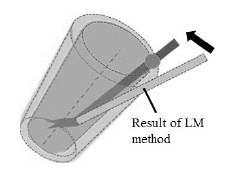
\includegraphics[width=0.6\textwidth]{figures/collision_avoidance.png}
            \caption{Relocation of the tool shaft with the automatic collision avoidance algorithm \cite{collisionAvoidanceNeuro}}
            \label{fig:gripper_design}
        \end{figure}
    
        \begin{block}{\LARGE Robot-Operation}
            \justifying  \normalsize 
            \begin{itemize}
                \item Teleoperated or fully-automated systems
                \item Higher accuracy
                \item Location independent
                \item Automatic collision avoidance \cite{collisionAvoidanceNeuro} and real-time tool detection \cite{retinal_tool_detector}
            \end{itemize}
        \end{block}

    \end{column}
    
    \begin{column}{0.45\textwidth}
        \begin{figure}
            \centering
            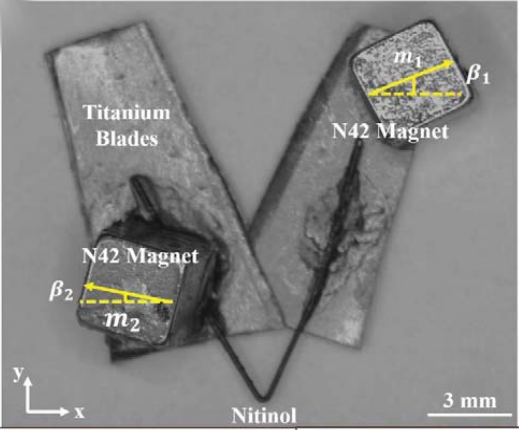
\includegraphics[width=0.6\textwidth]{figures/scissor_prototype.png}
            \caption{Prototype of a micro scissor \cite{ScissorActuation}}
            \label{fig:gripper_design}
        \end{figure}    
        
        \vspace*{100pt}
        
        \begin{block}{\LARGE Current state}
            \justifying \normalsize 
            \begin{itemize}
                \item Possible applications: Neurosurgery, Ophtalmic, Pregnancy Help
                \item Development of new tools to fit the micro surgery \cite{StiffnessTuning}\cite{ScissorActuation} \cite{MilliGripper}
                \item Can heal more diseases
            \end{itemize}
        \end{block}
        
        \vspace*{20pt}
        
        \begin{figure}
            \centering
            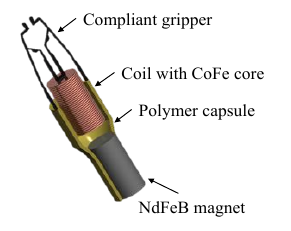
\includegraphics[width=0.8\textwidth]{figures/structure_gripper.png}
            \caption{Design of a milli gripper to rip tissue off \cite{MilliGripper}}
            \label{fig:duck3}
        \end{figure}
        
        \vspace*{40pt}
        
        \begin{block}{\LARGE Conclusion}
	        \justifying \normalsize 
	        \begin{itemize}
                \item Many advantages over manual surgeries
                \item First miniature robotic systems are commercially available
	            \item Current platforms have issues
	        \end{itemize}
        \end{block}
    
    \end{column}
    
\end{columns}

\begin{block}{References}
    \printbibliography
\end{block}

\end{frame}


\end{document}
	